\chapter{Web of Things}
\label{web-of-things}

\section{Web of Things vs Internet of Things}

\textbf{Internet of Things: una definizione} \\

Internet of Things è un sistema di oggetti fisici che possono essere
rilevati, monitorati, controllati o con cui si può interagire con
devices elettronici, che comunicano fra loro attraverso interfacce di rete
e, infine, che possono collegarsi a Internet.

C'è una nuova classe di oggetti che sta per entrare nelle nostre case:
le \textbf{Smart Things}. Una Smart Thing è un oggetto fisico ``digitalmente
aumentato'' con una o più delle seguenti caratteristiche:

\begin{itemize}
  \item Sensori (temperatura, luce, movimento, ecc.)
  \item Attuatori (displays, suoni, etc.)
  \item Proprietà computazionali (possono eseguire programmi)
  \item Interfacce di comunicazione (wired or wireless)
\end{itemize}

\begin{figure}[H]
  \centering
  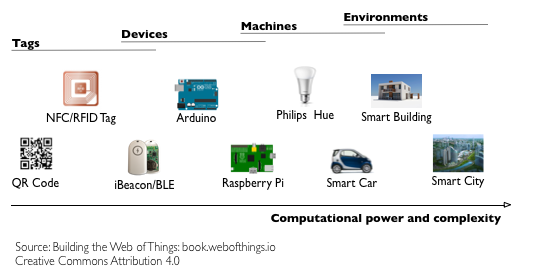
\includegraphics[scale=0.6]{iotland.png}
  \caption{Scenario IoT. IoT è una rete di oggetti collegati ad Internet.}
  \label{fig:iotland}
\end{figure}

Il nome ``Internet delle cose'' significa semplicemente che un oggetto (e i
suoi servizi o dati da/verso esso) può essere acceduto e processato da altre
applicazioni attraverso l'esistente infrastruttura di Internet.

Le limitazioni dell'IoT diventano evidenti non appena si vuole integrare
dispositivi di vari produttori in una singola applicazione o sistema.

\begin{figure}[H]
  \centering
  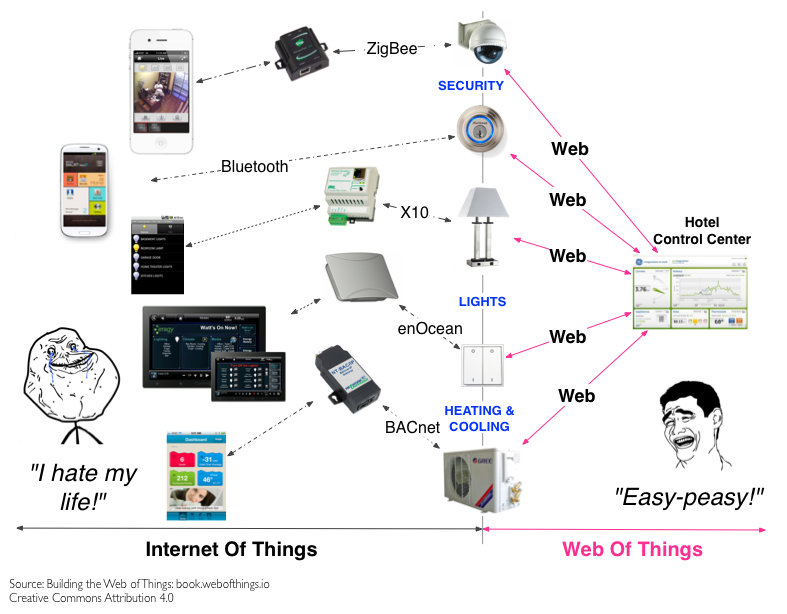
\includegraphics[scale=0.5]{integration_problem.png}
  \caption{Nell'IoT, oggi esistono centinaia di protocolli incompatibili.
Ciò rende l'integrazione di dati e servizi da vari dispositivi estremamente
complessa e costosa.}
  \label{fig:integration_problem}
\end{figure}

\subsection{Sfuggire al pattern ``un device, un protocollo, una sola app''}

Nel Web of Things (non IoT!), è possibile accedere a qualsiasi dispositivo
utilizzando protocolli web standard.

Collegare dispositivi eterogenei al Web rende la loro integrazione in sistemi
più ampi e/o applicazioni molto più semplice.

L'idea di applicare gli strumenti e le tecniche presenti nel
Web allo sviluppo di scenari IoT si chiama Web of Things.

Mentre IoT si occupa di risolvere problemi di rete, il Web of Things si basa
esclusivamente su protocolli e strumenti a livello di applicazione.

Mappare un qualsiasi dispositivo in un contesto Web rende agnostico il
Web of Things rispetto ai protocolli di livello fisico e di trasporto
utilizzati dai dispositivi.

\begin{figure}[H]
  \centering
  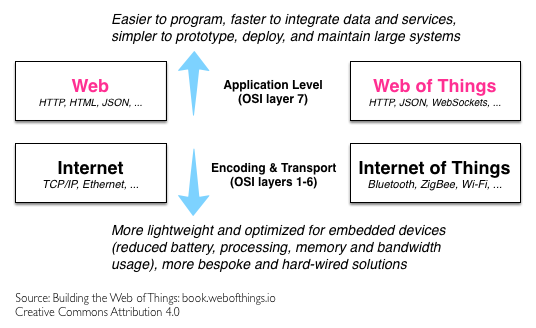
\includegraphics[scale=0.6]{iotstack.png}
  \caption{Il Web of Things riguarda solo il più alto livello OSI, che
gestisce applicazioni, servizi e dati.
Lavorare con un elevato livello di astrazione consente di collegare dati
e servizi da molti dispositivi indipendentemente dai veri e propri protocolli
di trasporto usati.
Al contrario, l'Internet of Things non sostiene un particolare protocollo a
livello di applicazione e di solito si concentra sugli strati inferiori dello
Stack OSI.}
  \label{fig:iotstack}
\end{figure}

\textbf{Lo scopo è quello di accedere alle cose in modo standardizzato e
trasparente.}

\begin{figure}[H]
  \centering
  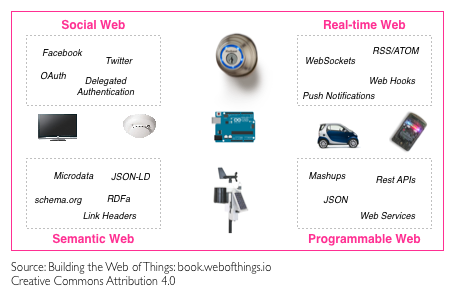
\includegraphics[scale=0.7]{iotweb.png}
  \caption{Il Web of Things è la capacità di utilizzare gli standard web moderni
direttamente su dispositivi embedded.}
  \label{fig:iotweb}
\end{figure}

Questo rende il Web il substrato ideale per la creazione di un'architettura
``universale'' e di Application Programming Interface (API) con cui gli oggetti possono
interagire.

In pratica, questo significa che l'utente può iniziare a interagire con gli oggetti
via Web

I dati real-time raccolti da sensori distribuiti possono essere facilmente
recuperati, elaborati e visualizzati in pagine Web utilizzando HTML, CSS e
JavaScript.

\begin{figure}[H]
  \centering
  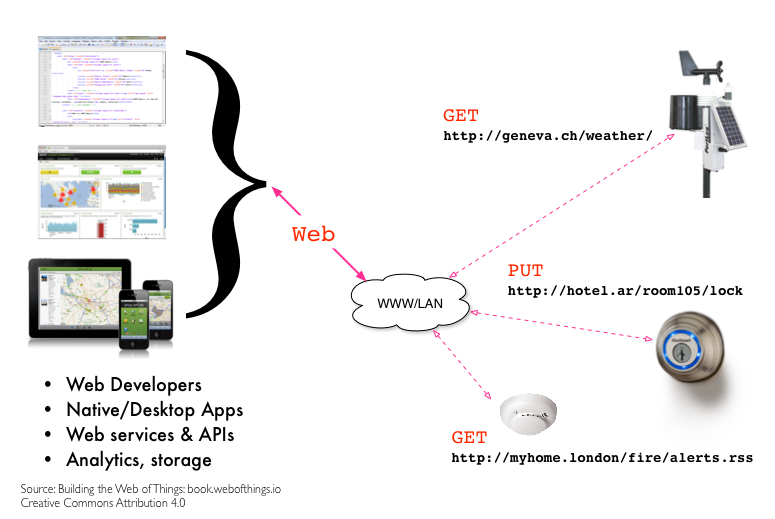
\includegraphics[scale=0.5]{iotrest.png}
  \caption{Un URL per ogni cosa e un'API RESTful.
Il Web delle cose consente agli sviluppatori e alle applicazioni di scambiare
dati con qualsiasi dispositivo che utilizza le richieste HTTP / WebSockets
standard, indipendentemente dal modo in cui il dispositivo è collegato.}
  \label{fig:iotrest}
\end{figure}

\textbf{MA} anche se i protocolli Web sono disponibili e utilizzabili per i
dispositivi IoT, possono essere troppo pesanti per alcune applicazioni di IoT.
Diamo un'occhiata ad altri protocolli.

\subsection{Not all speak HTTP}

\textbf{MQTT}\\

MQ Telemetry Transport (MQTT) is an open source protocol for constrained
devices and low-bandwidth, high-latency networks.
It has a publish/subscribe messaging transport that is extremely lightweight
and ideal for connecting small devices to constrained networks.
MQTT is bandwidth efficient, data agnostic, and has continuous session
awareness. It helps minimize the resource requirements for an IoT device,
while also attempting to ensure reliability and some degree of assurance of
delivery with grades of service.\\

\textbf{Properties:}

\begin{itemize}
  \item client/server model, where every sensor is a client and connects to a
server (a.k.a. broker)
  \item clients subscribe to topic channels of interest
  \item topic channels are hierarchical (e.g., room2BC/heating)
  \item 3 QoS Levels: ``Fire and forget'',  ``delivered at least once'' and
 ``delivered exactly once''.
  \item username/password authentication
  \item TCP over SSL/TLS
\end{itemize}

\textbf{CoAP}\\

The Constrained Application Protocol (CoAP) was designed for use with low-power
and constrained networks. CoAP is a RESTful protocol. It is semantically
aligned with HTTP, and even has a one-to-one mapping to and from HTTP.\\

\textbf{Properties:}

\begin{itemize}
  \item packets are much smaller than HTTP TCP flows
  \item simpler and faster to parse with small memory footprint
  \item over UDP, interoperates with HTTP and the RESTful web through simple
proxies
  \item client/server model where clients may GET, PUT, POST and DELETE
resources
  \item DTLS capable CoAP devices support RSA and AES or ECC and AES
\end{itemize}

\begin{figure}[H]
  \centering
  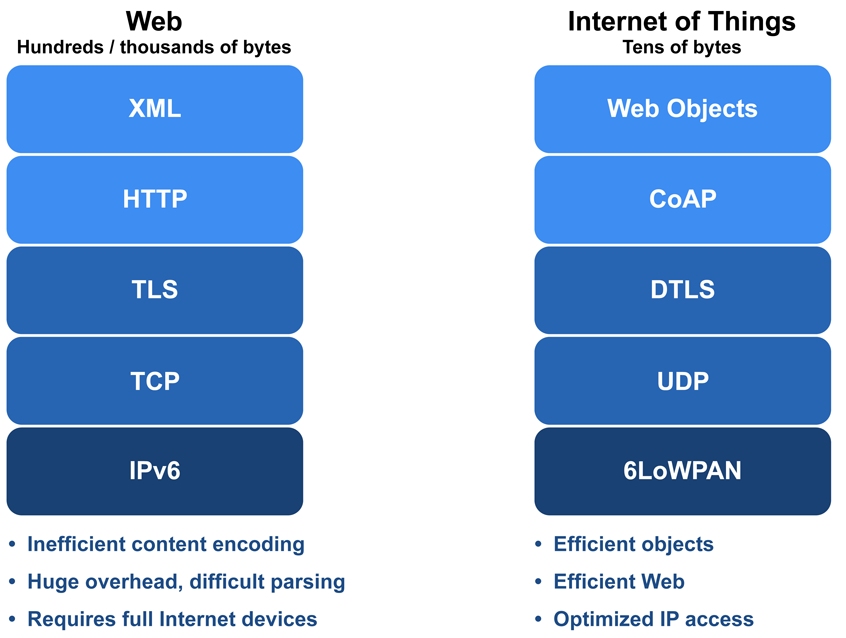
\includegraphics[scale=0.4]{protocol_comparison.png}
  \caption{On the left, the protocol stack for Web applications can easily
produce a data overhead of hundreds or thousands of bytes.
By comparison, IoT protocols are optimized for constrained devices and
networks, and produce a much smaller data overhead of tens of bytes.}
  \label{fig:protocol_comparison}
\end{figure}

\subsection{Integration Patterns}

\textbf{Direct Communication}

In the most straightforward case, a Web Thing is simply a Web API that Clients
send requests to.
The Client and the Web Thing can be on the same network or on different
networks.

\begin{figure}[H]
  \centering
  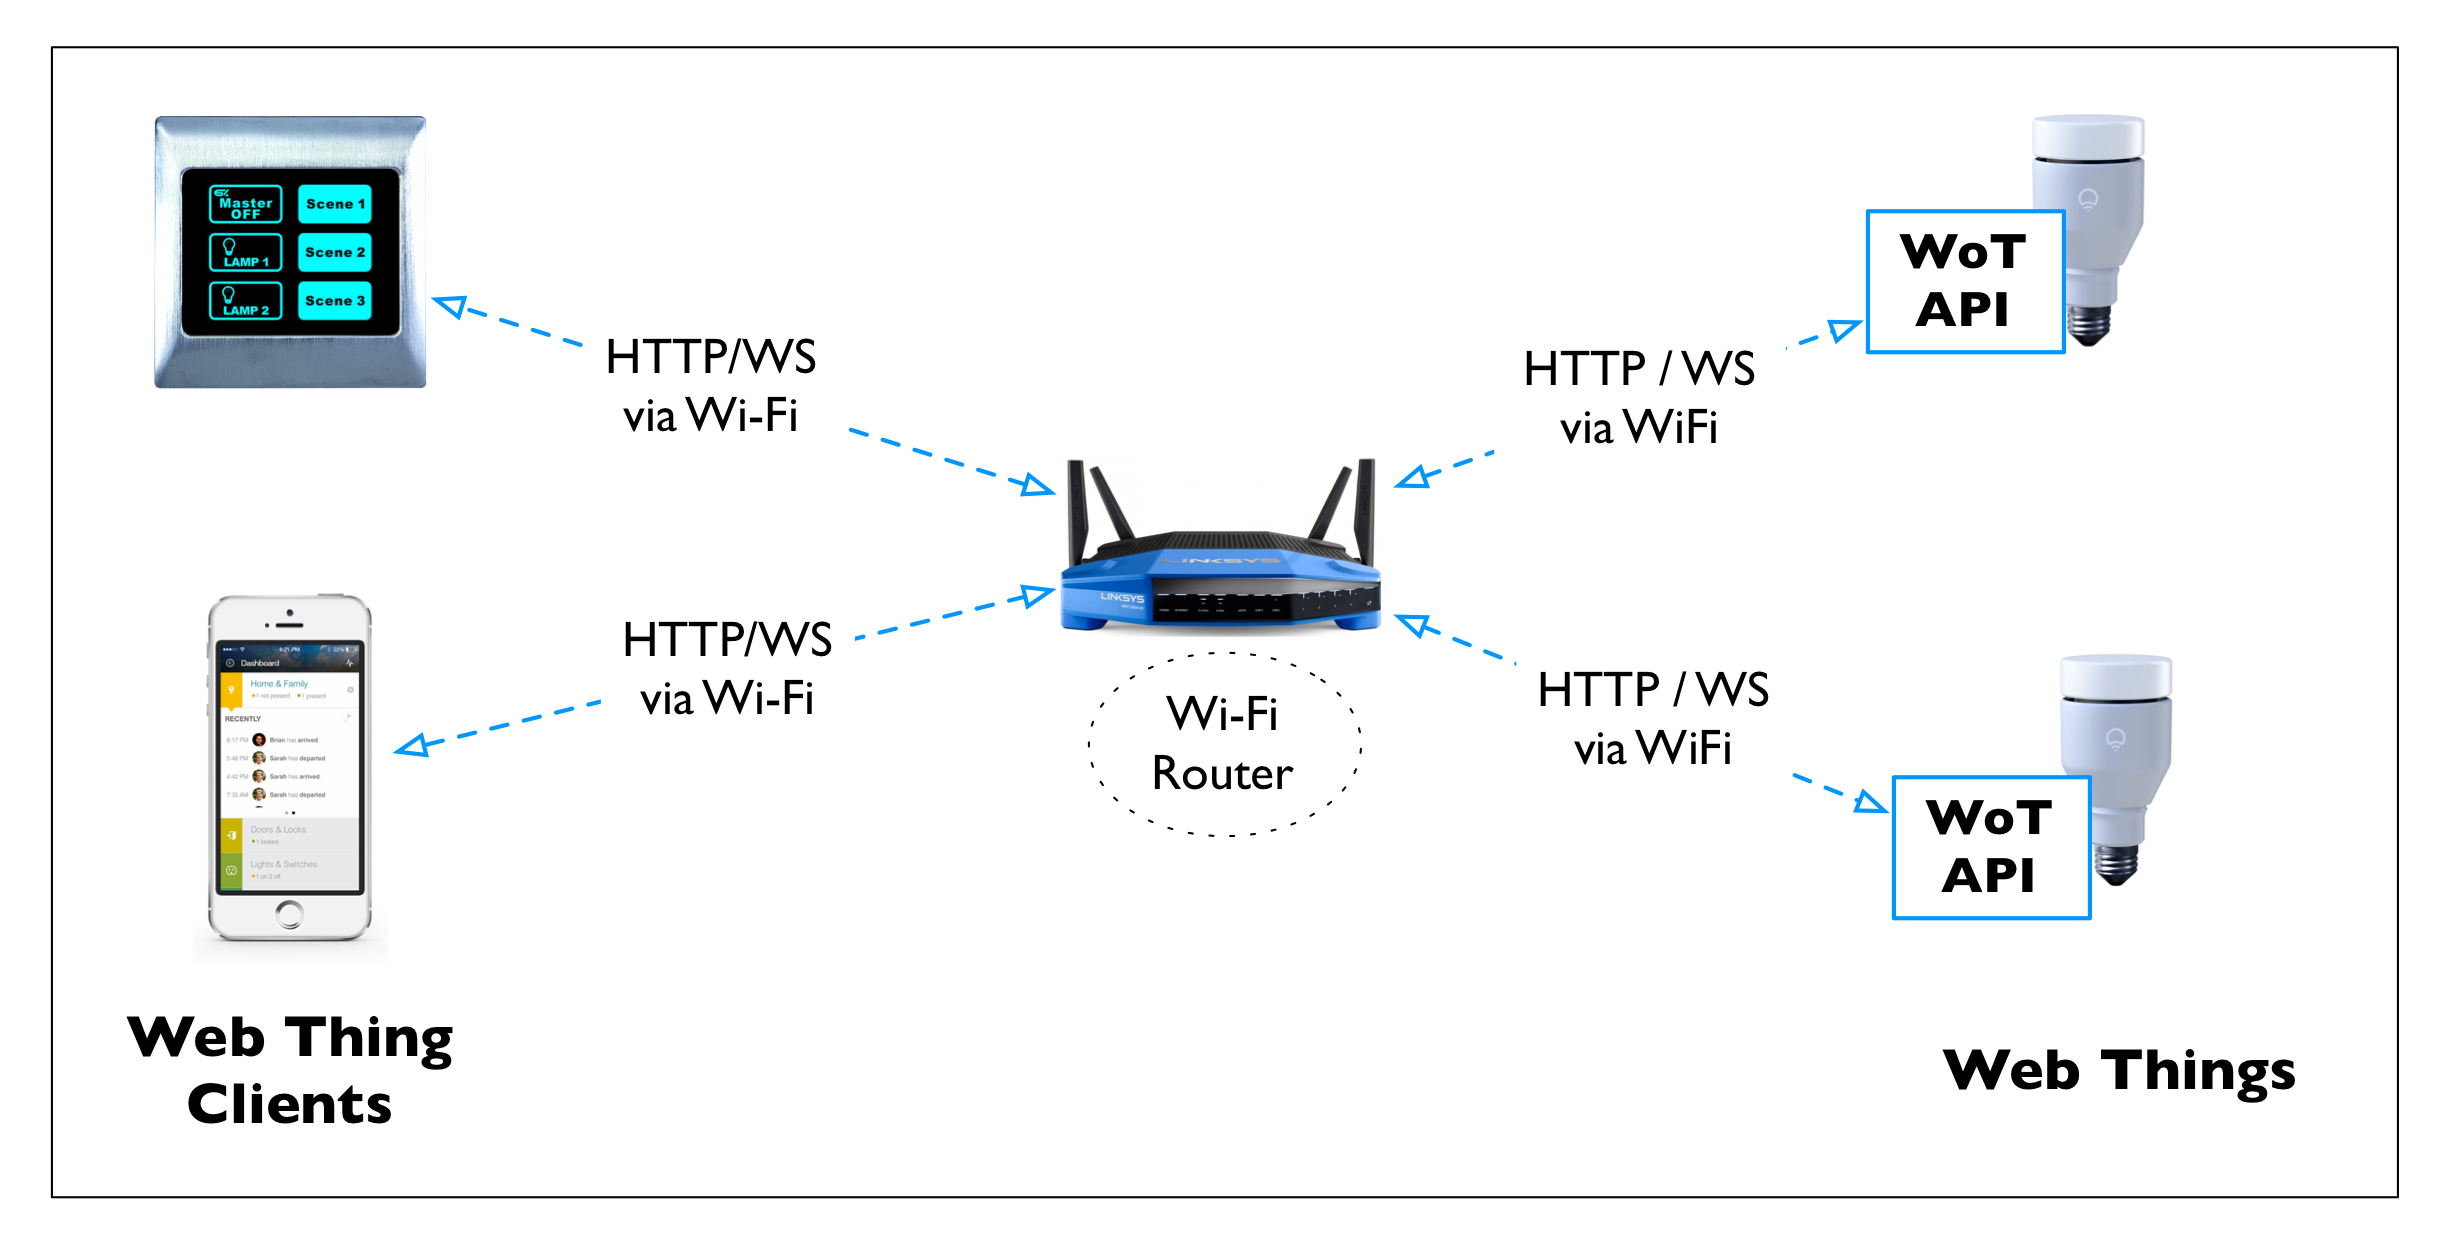
\includegraphics[scale=0.5]{direct_communication.png}
  \caption{Direct connectivity between a Client and a Web Thing}
  \label{fig:direct_communication}
\end{figure}

\textbf{Gateway}

Gateway-based connectivity is used when a Thing cannot offer a Web API
directly.

In this case an intermediate Web Thing - the gateway - exposes a Web API on the
Thing's behalf (per conto di).
The Web Thing therefore acts as a proxy for the Thing (or gateway depending on
the complexity/layer of the translation).

\begin{figure}[H]
  \centering
  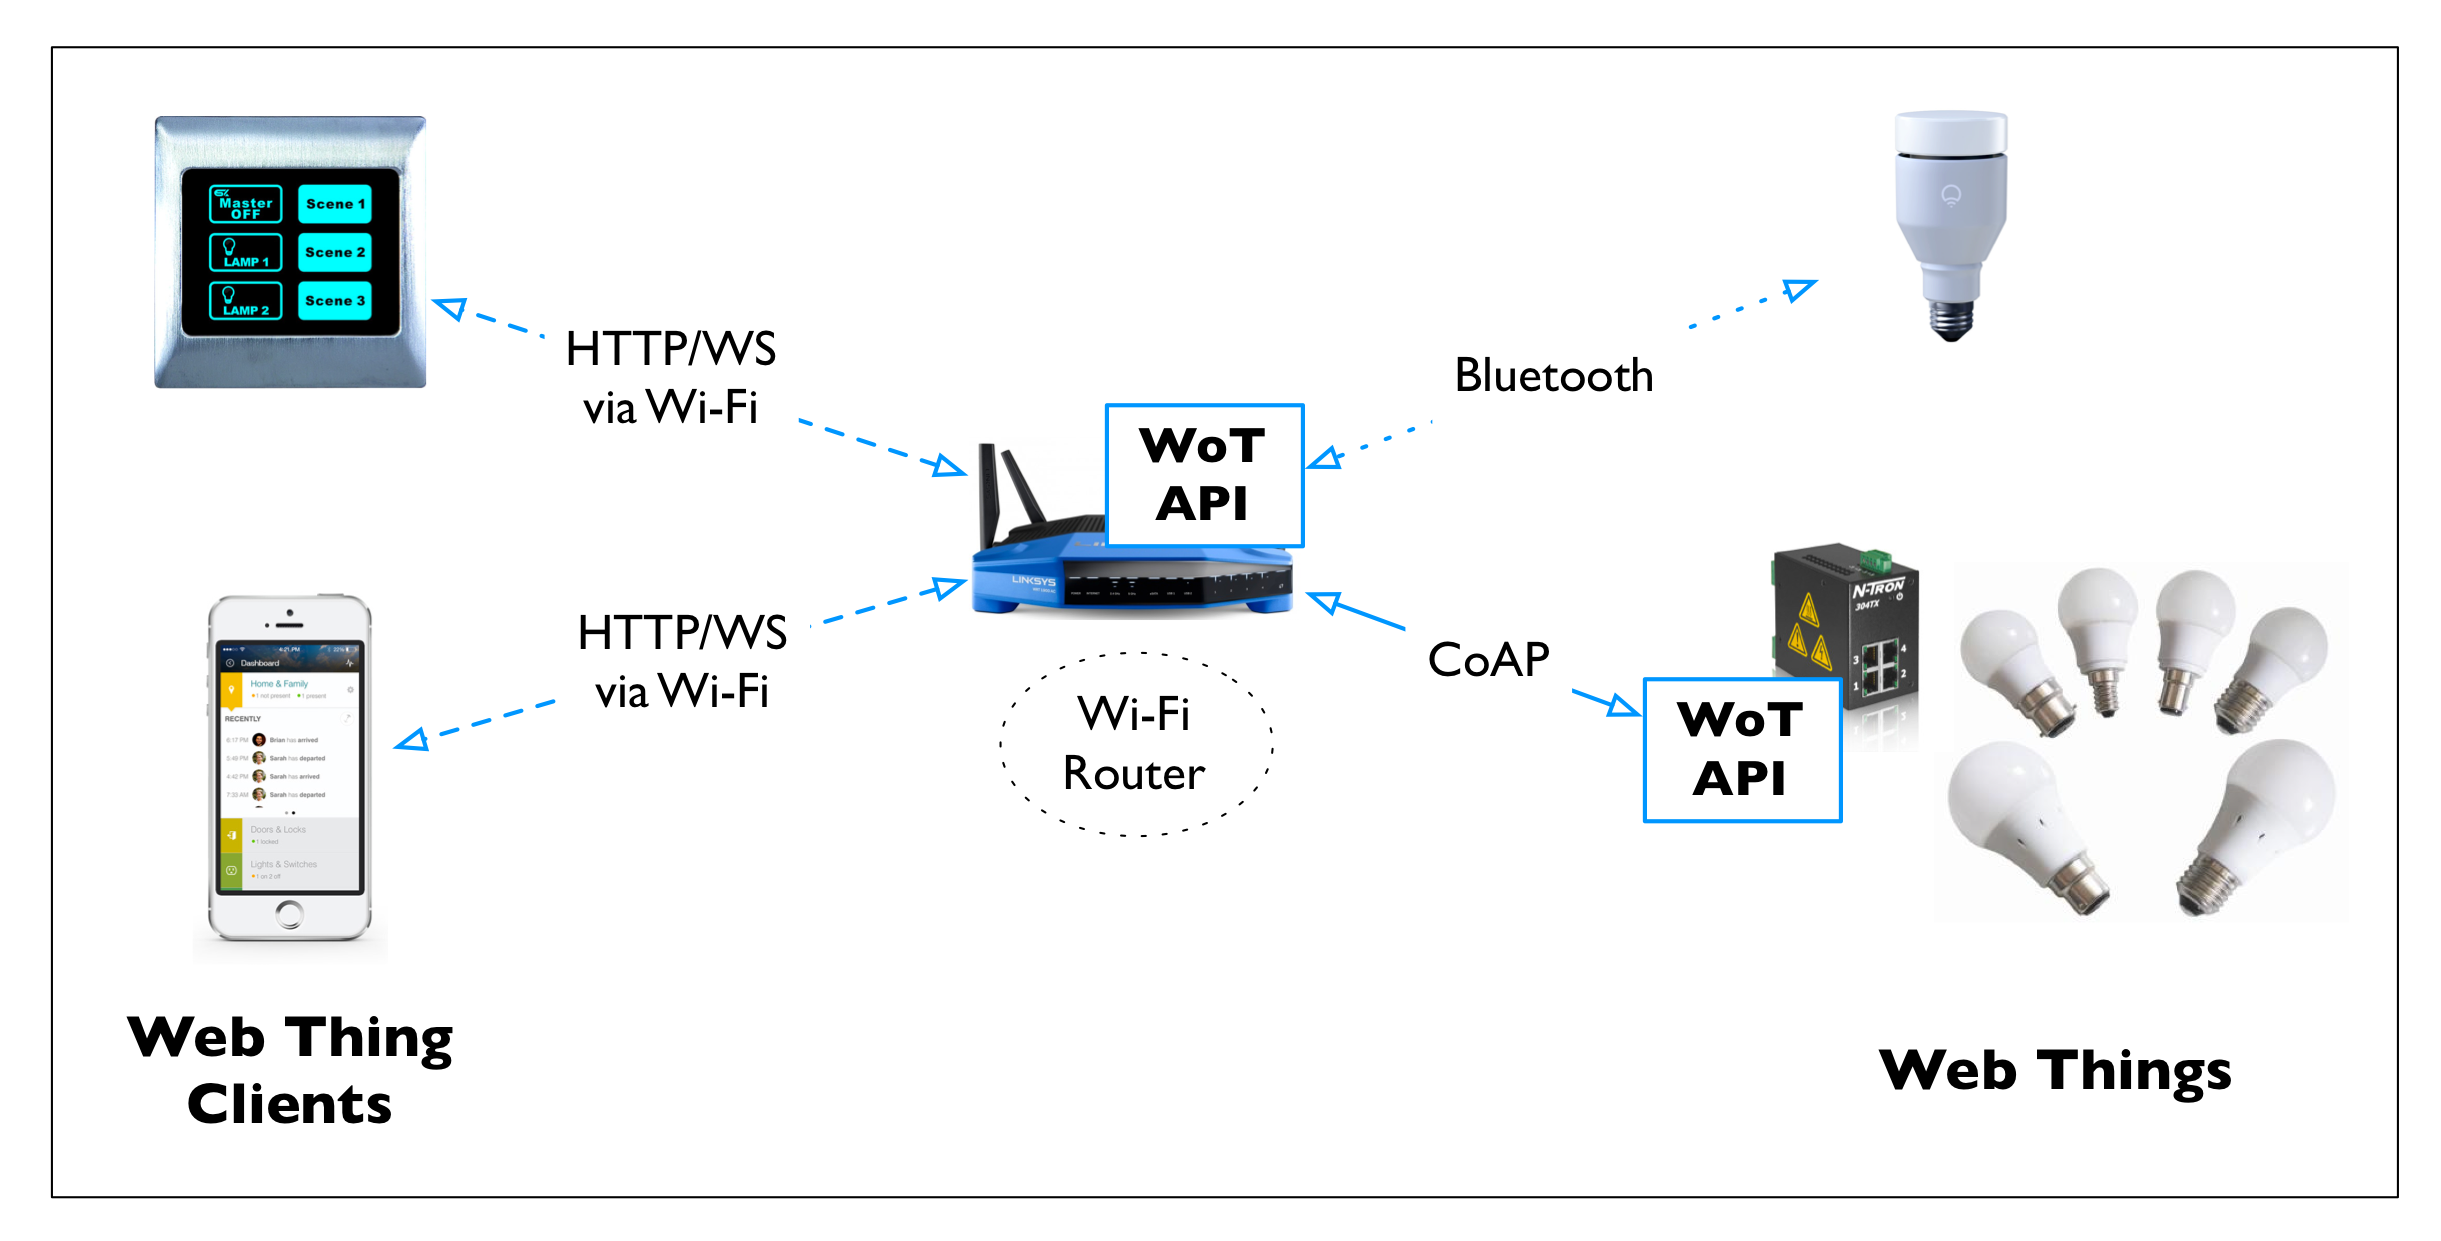
\includegraphics[scale=0.5]{gateway.png}
  \caption{Gateway-based connectivity between a Client and a Web Thing}
  \label{fig:gateway}
\end{figure}

\textbf{Cloud}

This third case is similar to the previous case. However, this time the gateway
is a cloud service.

\begin{figure}[H]
  \centering
  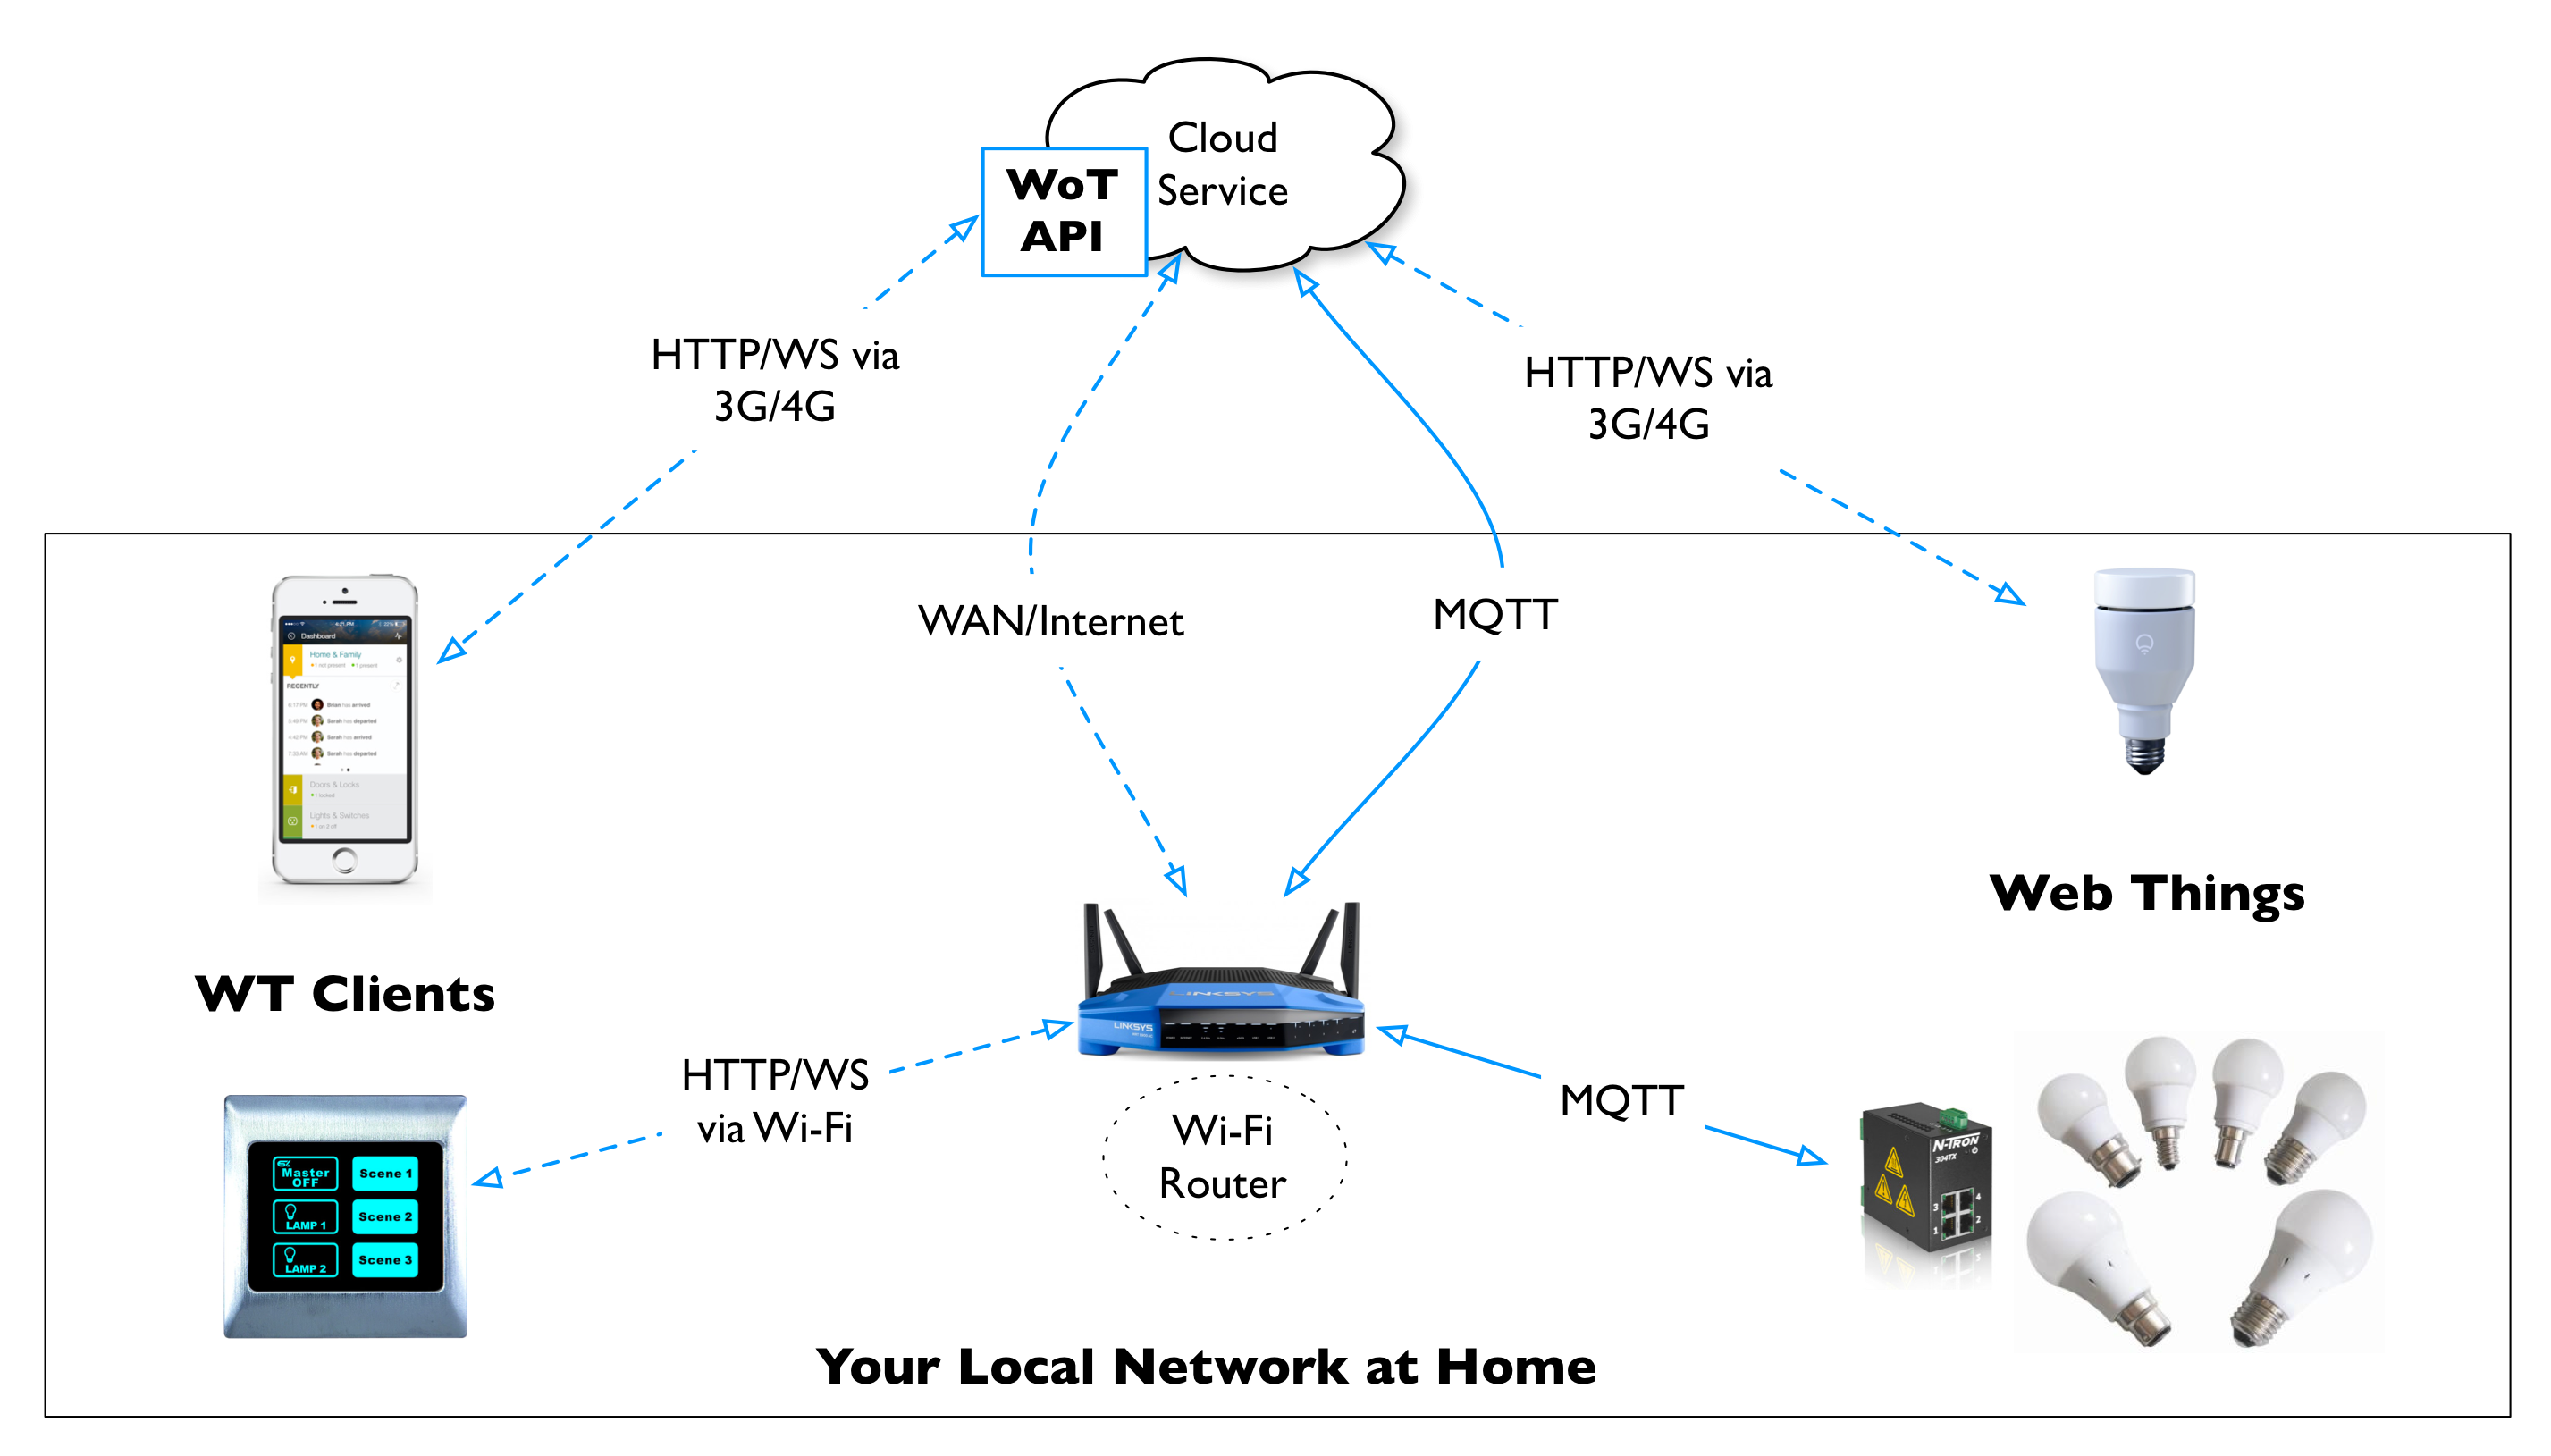
\includegraphics[scale=0.5]{cloud.png}
  \caption{Cloud-based connectivity between a Client and a Web Thing}
  \label{fig:cloud}
\end{figure}

\subsection{Web of Things Architecture}

While there are ongoing efforts to standardise it, the Web of Things is a set 
of best practices that can be classified according to the Web of Things
architecture.
The architecture proposes four main layers that are used as a framework to
classify the different patterns and protocols involved.

\begin{figure}[H]
  \centering
  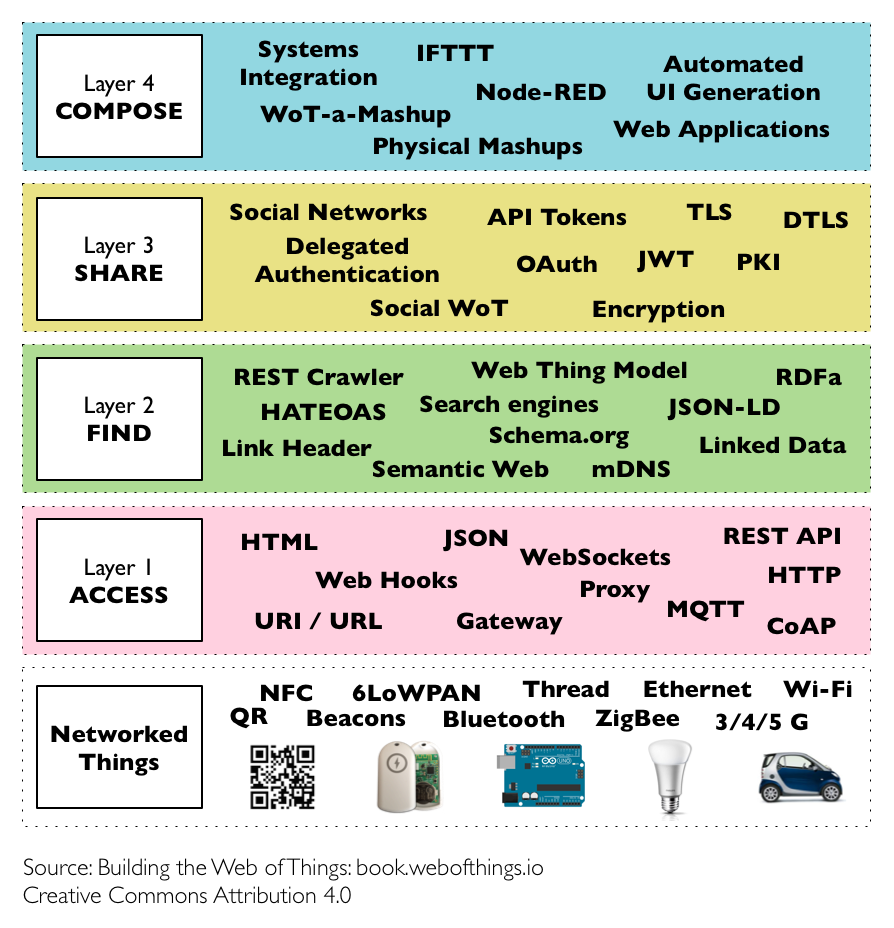
\includegraphics[scale=0.5]{wotarchitecture.png}
  \caption{Web of Things Architecture}
  \label{fig:wotarchitecture}
\end{figure}

\textbf{Accessibility layer}\\

This layer deals with the access of things to the
Internet and ensure they expose their services via Web APIs
(already discussed in the previous sections of this chapter).\\

\textbf{Findability layer}\\

Marking things accessible via an HTTP and WebSocket API is great but it doesn't
mean applications can really  ``understand'' what the Thing is, what data or
services it offers, and so on.

This is where the second layer – Find – becomes interesting.
This layer ensures that your Thing can not only be easily used by other HTTP
clients but can also be findable and automatically usable by other WoT
applications.

The approach here is to reuse web semantic standards to describe things and
their services.

This enables searching for things through search engines and other web indexes
as well as the automatic generation of user interfaces or tools to interact
with Things.\\

\textbf{Sharing layer}\\

The Internet of Things will only blossom (fiorirà) if Things have a way to
securely share data across services.

This is the responsibility of the Share layer, which specifies how the data
generated by Things can be shared in an efficient and secure manner over
the web.

At this level, another batch of Web protocols help.
First, TLS, the protocol that makes transactions on the Web secure.
Then, techniques such as delegated web authentication mechanisms like OAuth
which can be integrated to our Things' APIs. Finally, we can also use social
networks to share Things and their resources to create a Social Web of
Things.\\

\textbf{Composition layer}\\

Finally, once Things are on the Web (layer 1) where they can be found by humans
and machines (layer 2) and their resources can be shared securely with others
(layer 3), it's time to look at how to build large-scale, meaningful
applications for the Web of Things. In other words, we need to understand the
integration of data and services from heterogeneous Things into an immense
ecosystem of web tools such as analytics software and mashup platforms.
Web tools at the Compose layer range from web toolkits - for example,
JavaScript SDKs offering higher-level abstractions - to dashboards with
programmable widgets, and finally to physical mashup tools such as Node-RED as
shown below.

\begin{figure}[H]
  \centering
  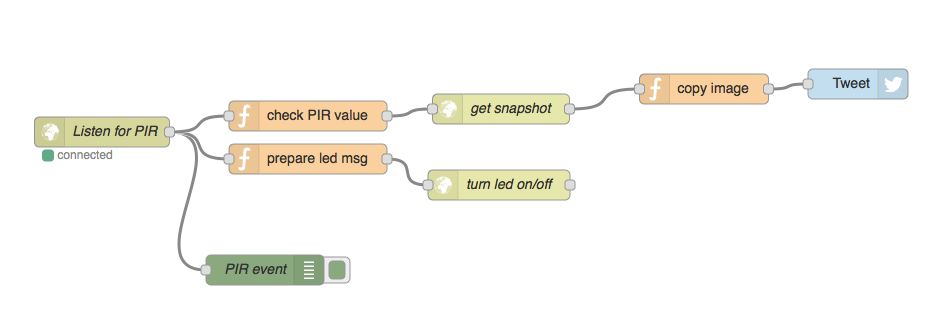
\includegraphics[scale=0.4]{nodered.png}
  \caption{A Physical Mashup with Node-RED;
Monitor a process / sensor;
Automatic control of heating system;}
  \label{fig:nodered}
\end{figure}

\subsubsection{Conclusion}

The Web of Things is a high-level application protocol designed to maximize
interoperability in the IoT. Web technologies are widely popular and offer all
the flexibility and features needed for the majority of future IoT
applications, including discovery, security, and real-time messaging.\\

\textbf{Sources:}\\

A mix of:

\begin{itemize}
  \item Course slides
  \item \url{http://webofthings.org/2016/01/23/wot-vs-iot-12/}
  \item \url{http://webofthings.org/2017/04/08/what-is-the-web-of-things/}
  \item \url{https://www.micrium.com/iot/internet-protocols/}
  \item \url{https://www.w3.org/blog/wotig/}
\end{itemize}
